\documentclass[english]{beamer}\usepackage[]{graphicx}\usepackage[]{color}
%% maxwidth is the original width if it is less than linewidth
%% otherwise use linewidth (to make sure the graphics do not exceed the margin)
\makeatletter
\def\maxwidth{ %
  \ifdim\Gin@nat@width>\linewidth
    \linewidth
  \else
    \Gin@nat@width
  \fi
}
\makeatother

\definecolor{fgcolor}{rgb}{0.345, 0.345, 0.345}
\newcommand{\hlnum}[1]{\textcolor[rgb]{0.686,0.059,0.569}{#1}}%
\newcommand{\hlstr}[1]{\textcolor[rgb]{0.192,0.494,0.8}{#1}}%
\newcommand{\hlcom}[1]{\textcolor[rgb]{0.678,0.584,0.686}{\textit{#1}}}%
\newcommand{\hlopt}[1]{\textcolor[rgb]{0,0,0}{#1}}%
\newcommand{\hlstd}[1]{\textcolor[rgb]{0.345,0.345,0.345}{#1}}%
\newcommand{\hlkwa}[1]{\textcolor[rgb]{0.161,0.373,0.58}{\textbf{#1}}}%
\newcommand{\hlkwb}[1]{\textcolor[rgb]{0.69,0.353,0.396}{#1}}%
\newcommand{\hlkwc}[1]{\textcolor[rgb]{0.333,0.667,0.333}{#1}}%
\newcommand{\hlkwd}[1]{\textcolor[rgb]{0.737,0.353,0.396}{\textbf{#1}}}%
\let\hlipl\hlkwb

\usepackage{framed}
\makeatletter
\newenvironment{kframe}{%
 \def\at@end@of@kframe{}%
 \ifinner\ifhmode%
  \def\at@end@of@kframe{\end{minipage}}%
  \begin{minipage}{\columnwidth}%
 \fi\fi%
 \def\FrameCommand##1{\hskip\@totalleftmargin \hskip-\fboxsep
 \colorbox{shadecolor}{##1}\hskip-\fboxsep
     % There is no \\@totalrightmargin, so:
     \hskip-\linewidth \hskip-\@totalleftmargin \hskip\columnwidth}%
 \MakeFramed {\advance\hsize-\width
   \@totalleftmargin\z@ \linewidth\hsize
   \@setminipage}}%
 {\par\unskip\endMakeFramed%
 \at@end@of@kframe}
\makeatother

\definecolor{shadecolor}{rgb}{.97, .97, .97}
\definecolor{messagecolor}{rgb}{0, 0, 0}
\definecolor{warningcolor}{rgb}{1, 0, 1}
\definecolor{errorcolor}{rgb}{1, 0, 0}
\newenvironment{knitrout}{}{} % an empty environment to be redefined in TeX

\usepackage{alltt}
%% The most common packages are already included in:
\usetheme{biostat}
%%%%%%%%%%%%%%%%%%%%%%%%%%%%%%%%%%%%%%%%%%%%%%%%%%%%%%%% 
\usepackage{amsmath,amsfonts,tikz, amssymb}
\usetikzlibrary{trees}

%% Header data: (adjust to your needs:
\def\uzhunit{Biostatistics}             %% if (not) needed comment/uncomment
%\def\uzhunitext{STA480}

\title{Publication Bias in Cochrane Meta-Analyses}%[Publication Bias]
%% Optional Argument in [Brackets]: Short Title for Footline

%% The following are all optional, simply comment them
%\subtitle{Publication Bias in the Cochrane Libary}
%\institute{Biostatistics Journal Club}  %% optional
\author{Giuachin Kreiliger}
\date{\today}

\usepackage{xifthen}            % for \isempty
\usepackage{array}
\usepackage{amssymb}

%%%%%%%%%%%%%%%%%%%%%%%%%%%%% Kommentare %%%%%%%%%%%%%%%%%%%%%%%%%%%%%

% Zum Kommentieren
\newcommand{\komm}[1]{%
  \marginpar{\fbox{% mit Rahmen
    \begin{minipage}{1.4cm}  % Für automatischen Zeilenumbruch im Kommentar
      {\footnotesize\bfseries #1}
    \end{minipage}
  }
 }
} 


% Zum Auskommentieren
\newcommand{\blanco}[1]{  } 
%\usepackage[sumlimits, intlimits, namelimits]{amsmath} 

%%%%%%%%%%%%%%%%%%%%%%%%%%% Formatierung %%%%%%%%%%%%%%%%%%%%%%%%%%%%%%

%\newcommand{\alert}{}
\newcommand{\gqs}{}

% für englische Begriffe: Achtung, falls sich ein Wort anschließt so:
% \english{engWord}{}, d.h. Klammern nicht vergessen  
\newcommand{\english}[1]{\glqq #1\grqq}

% für lateinische Begriffe, z. B. a posteriori, ad hoc, etc
\newcommand{\latin}[1]{\textit{#1}}

% für Definitionen
\newcommand{\define}[1]{\emph{#1}} % jetzt ohne index, das muss manuell gemacht werden

% angeben von Personennamen
\newcommand{\name}[1]{\textsc{#1}} 

% Abkürzungen richtig setzen ("z.B.") 
\newcommand{\abks}[1]{\mbox{\scriptsize #1}\xdot}
\newcommand{\abk}[1]{\mbox{#1}\xdot}
\DeclareRobustCommand\xdot{\futurelet\token\Xdot}
\def\Xdot{%
  \ifx\token\bgroup.%
  \else\ifx\token\egroup.%
  \else\ifx\token\/.%
  \else\ifx\token\ .%
  \else\ifx\token!.%
  \else\ifx\token,.%
  \else\ifx\token:.%
  \else\ifx\token;.%
  \else\ifx\token?.%
  \else\ifx\token/.%
  \else\ifx\token'.%
  \else\ifx\token).%
  \else\ifx\token-.%
  \else\ifx\token+.%
  \else\ifx\token~.%
  \else\ifx\token.%
  \else.\ %
  \fi\fi\fi\fi\fi\fi\fi\fi\fi\fi\fi\fi\fi\fi\fi\fi%
}

\newcommand{\etc}{\abk{etc}}
\newcommand{\Prof}{\abk{Prof}}
\newcommand{\Dr}{\abk{Dr}}
\newcommand{\vgl}{\abk{vgl}}
\newcommand{\zB}{\abk{z.\,B}}
\newcommand{\bzgl}{\abk{bzgl}}
\newcommand{\bzw}{\abk{bzw}}
\newcommand{\dH}{\abk{d.\,h}}
\newcommand{\ua}{\abk{u.\,a}}
\newcommand{\ca}{\abk{ca}}
\newcommand{\ggf}{\abk{ggf}}
\newcommand{\eg}{\abk{\latin{e.\,g}}}
\newcommand{\ie}{\abk{\latin{i.\,e}}}
\newcommand{\cf}{\abk{\latin{cf}}}

% Grafikskalierung
\newcommand{\graphicSize}[1]{\setkeys{Gin}{width = #1\textwidth, keepaspectratio}}
\newcommand{\fullwidth}{\setkeys{Gin}{width = \textwidth, keepaspectratio}}

\newlength{\halbebreite}
\setlength{\halbebreite}{\textwidth / 2 - 0.5cm}
\newcommand{\halfwidth}{\setkeys{Gin}{width = \halbebreite, keepaspectratio}}

% Referenzierung von Listenelementen
%\newcommand{\subref}[1]{\ref{#1})}

%%%%%%%%%%%%%%%%%%%%%%%%%%%%%% Befehle %%%%%%%%%%%%%%%%%%%%%%%%%%%%%%%

% Verteilungen (- bedeutet: im Appendix eingetragen)
\DeclareMathOperator{\Ber}{B} % Bernoulli - 
% \DeclareMathOperator{\Bin}{Bin} % Binomial Distribution - 
\DeclareMathOperator{\Cauchy}{C} % Cauchy Distribution (special Student -
                                % dist.) 
\DeclareMathOperator{\Par}{Par} % Pareto Distribution
\DeclareMathOperator{\Mult}{M} % Multinomialverteilung - 
\DeclareMathOperator{\NegBin}{NBin} % Negative Binomial - 
\DeclareMathOperator{\HypGeom}{HypGeom} % Hypergeometric Distribution - 
\DeclareMathOperator{\NCHypGeom}{NCHypGeom} % Noncentral hypergeometric Distribution - 
\DeclareMathOperator{\Geom}{Geom} % Geometric Distribution - 
\DeclareMathOperator{\Po}{Po} % Poisson Distribution - 
% \DeclareMathOperator{\Exp}{Exp} % Exponential Distribution -
\DeclareMathOperator{\Nor}{N} % Normal -
\DeclareMathOperator{\LN}{LN} % Log-Normal - 
\DeclareMathOperator{\HN}{HN} % Halb-Normal - 
\DeclareMathOperator{\FN}{FN} % gefaltet Normal - 
\DeclareMathOperator{\Gumbel}{Gu} % Gumbel - 
% \DeclareMathOperator{\F}{F} % F - 
\DeclareMathOperator{\stud}{t} % Student - 
\DeclareMathOperator{\Stud}{\stud}  
\DeclareMathOperator{\Log}{Log} % Logistische Verteilung - 
\DeclareMathOperator{\Uni}{U} % Uniform -
\DeclareMathOperator{\Ga}{G} % Gamma - 
% \DeclareMathOperator{\IG}{IG} % Invers-Gamma - 
\DeclareMathOperator{\Gg}{Gg} % Gamma-Gamma - 
\DeclareMathOperator{\Be}{Be} % Beta - 
\DeclareMathOperator{\BeB}{BeB} % Beta-Binomial - 
\DeclareMathOperator{\PoG}{PoG} % Poisson-Gamma - 
\DeclareMathOperator{\Wb}{Wb} % Weibull - 
\DeclareMathOperator{\Dir}{D} % Dirichlet - 
\DeclareMathOperator{\Wish}{Wi} % Wishart 
\DeclareMathOperator{\InvWish}{IWi} % Inverse Wishart
\DeclareMathOperator{\MultDir}{MD} % Multinomial-Dirichlet -
\DeclareMathOperator{\NoG}{NG} % Normal-Gamma - 

% Operatoren
\DeclareMathOperator{\Var}{Var} % Varianz
% \DeclareMathOperator{\E}{\mathsf{E}} % Erwartungswert
\newcommand{\KLD}[2]{\mathsf{D}(#1 \parallel{} #2)} % new KL discrepancy
\DeclareMathOperator{\Cov}{Cov} % Covariance
\DeclareMathOperator{\Corr}{Corr} % Correlation 
\DeclareMathOperator{\se}{se}   % standard error
\DeclareMathOperator{\sign}{sign} % signum
\DeclareMathOperator{\logit}{logit} % logit-Funktion
\DeclareMathOperator{\Mod}{Mod} % Modus
\DeclareMathOperator{\Med}{Med} % Median
% \DeclareMathOperator{\diag}{diag} % Diagonalmatrix
% \DeclareMathOperator{\trace}{tr} % Spur
\renewcommand{\P}{\operatorname{\mathsf{Pr}}} % Wahrscheinlichkeitsmaß
%\newcommand{\p}{\operatorname{\mathsf{p}}} % Density function
% \newcommand{\p}{f}%{\operatorname{{p}}} % Density function
% \newcommand{\B}{\operatorname{{B}}} % Beta function
%\newcommand{\Lik}{\operatorname{\mathsf{L}}} % Probability/Density function
\newcommand{\Lik}{L} % Probability/Density function
\DeclareMathOperator{\dotcup}{\dot{\cup}} % disjunkte Vereinigung
% \DeclareMathOperator{\arctanh}{arctanh} % arcus tangens hyperbolicus
% \DeclareMathOperator*{\argmax}{arg\,max} % argument which maximises
% \DeclareMathOperator*{\argmin}{arg\,min} % argument which minimises

\DeclareMathOperator{\BS}{BS} % Brier Score
\DeclareMathOperator{\AS}{AS} % Absolute Score
\DeclareMathOperator{\CRPS}{CRPS} % CRPS
\DeclareMathOperator{\LS}{LS} % Logarithmic Score
\DeclareMathOperator{\SPE}{SPE} % Squared prediction error
\DeclareMathOperator{\SC}{SC} % Sander's calibration
\DeclareMathOperator{\MR}{MR} % Murphy resolution
\DeclareMathOperator{\AUC}{AUC} % Area under the curve
\DeclareMathOperator{\BF}{BF} % Bayes factor
\DeclareMathOperator{\mBF}{mBF} % minimum Bayes factor



% Zum Angeben von Funktionen
\newcommand{\funktion}[5]{%
	\begin{tabular}[t]{lrcl}
	$#1$~: & $#2$ & $\longrightarrow$ & $#3$\\
	& $#4$ & $\longmapsto$ & $#5$
	\end{tabular}}

% für Pfeil mit Erklärung unter einem Formelteil
\newcommand{\underarrow}[2]{%
 \underset{\begin{subarray}{c} \uparrow\\ #1 \end{subarray}}{#2}%
}

% Text über =
\newcommand{\overequal}[1]{\overset{\text{#1}}{=}}

% partielle Abl. von #2 nach #3 mit optionalem Parameter #1 für wievielte Ableitung (default 1)
\newcommand{\partialv}[3][1]{%
% \ifthenelse{#1 = 1}{\frac{\partial\,#2}{\partial\,#3}}{\frac{\partial^{#1} #2}{\partial\,#3^{#1}}}
\ifthenelse{#1 = 1}{\frac{\partial #2}{\partial #3}}{\frac{\partial^{#1} #2}{\partial #3^{#1}}}
} 

% Abl. von #2 nach Skalar #3 mit optionalem Parameter #1 für wievielte Ableitung (default 1)
\newcommand{\partials}[3][1]{%
%% \ifthenelse{#1 = 1}{\frac{d\,#2}{d\,#3}}{\frac{d^{#1} #2}{d\,#3^{#1}}}
\ifthenelse{#1 = 1}{\frac{d #2}{d #3}}{\frac{d^{#1} #2}{d #3^{#1}}}
} 

% partielle Abl. mit separatem Bruch für "nach einem Skalar" mit optionalem Parameter #1 für
% wievielte Ableitung (default 1) 
\newcommand{\dseps}[2][1]{%
% \ifthenelse{#1 = 1}{\frac{d}{d\,#2}}{\frac{d^{#1}}{d\,#2^{#1}}}
\ifthenelse{#1 = 1}{\frac{d}{d #2}}{\frac{d^{#1}}{d #2^{#1}}}
}

% partielle Abl. mit separatem Bruch mit optionalem Parameter #1 für
% wievielte Ableitung (default 1) 
\newcommand{\dsepv}[2][1]{%
% \ifthenelse{#1 = 1}{\frac{\partial\,}{\partial\,#2}}{\frac{\partial^{#1}}{\partial\,#2^{#1}}}
\ifthenelse{#1 = 1}{\frac{\partial}{\partial #2}}{\frac{\partial^{#1}}{\partial #2^{#1}}}
}

%%%%%%%%%%%%%%%%%%%%%%%%%%%%%% Abkürzungen %%%%%%%%%%%%%%%%%%%%%%%%%%%

% Mengen
\newcommand{\mcf}{\mathcal{F}}
\newcommand{\ve}{\varepsilon}
% \newcommand{\C}{\mathbb{C}}
\newcommand{\R}{\mathbb{R}}
% \newcommand{\Q}{\mathbb{Q}}
% \newcommand{\Z}{\mathbb{Z}}
% \newcommand{\N}{\mathbb{N}}
% \newcommand{\0}{\emptyset}
% \newcommand{\Tau}{\mathcal{T}}

% Quer-Versionen
\newcommand{\deltaq}{\bar{\delta}}
\newcommand{\xq}{\bar{x}}
\newcommand{\Xq}{\bar{X}}
\newcommand{\yq}{\bar{y}}
\newcommand{\Yq}{\bar{Y}}
\newcommand{\eq}{\bar{e}}

% Dach-Versionen
\newcommand{\xd}{\hat{x}}
\newcommand{\Xd}{\hat{X}}
\newcommand{\yd}{\hat{y}}
\newcommand{\Yd}{\hat{Y}}
\newcommand{\bd}{{\hat{\beta}}}
\newcommand{\ad}{{\hat{\alpha}}}
\newcommand{\pid}{\hat{\pi}}
\newcommand{\sd}{{\hat{\sigma}}}
\newcommand{\sda}{\hat{\sigma}_{\hat{\alpha}}}
\newcommand{\sdb}{\hat{\sigma}_{\hat{\beta}}}

% \newcommand{\ml}[2][1]{% % für Maximum-Likelihood-Schätzer von #1
% \ifthenelse{#1 = 1}%
%  {\hat{#2}_{\scriptscriptstyle{\mathrm{ML}}}}% 
%  {\hat{#2}^{#1}_{\scriptscriptstyle{\mathrm{ML}}}}% z.B. für sigmadach^2
% }
\newcommand{\map}[2][0]{% % für MAP-Schätzer von #1
\ifthenelse{#1 = 0}%
 {\hat{#2}_{\scriptscriptstyle{\mathrm{MAP}}}}% 
 {\hat{#2}_{{\scriptscriptstyle{\mathrm{MAP}}_{#1}}}}% z.B. für sigmadach^2
}
\newcommand{\mpm}[2][0]{% % für MPM-Schätzer von #1
\ifthenelse{#1 = 0}%
 {\hat{#2}_{\scriptscriptstyle{\mathrm{MPM}}}}% 
 {\hat{#2}_{{\scriptscriptstyle{\mathrm{MPM}}_{#1}}}}% z.B. für sigmadach^2
}

%% \newcommand{\ml}[2][1]{% % für Maximum-Likelihood-Schätzer von #1
%% \ifthenelse{#1 = 1}%
%%  {\hat{#2}_{\scriptscriptstyle{\text{ML}}}}% 
%%  {\hat{#2}^{#1}_{\scriptscriptstyle{\text{ML}}}}% z.B. für sigmadach^2
%% }
%% \newcommand{\map}[2][0]{% % für MAP-Schätzer von #1
%% \ifthenelse{#1 = 0}%
%%  {\hat{#2}_{\scriptscriptstyle{\text{MAP}}}}% 
%%  {\hat{#2}_{{\scriptscriptstyle{\text{MAP}}_{#1}}}}% z.B. für sigmadach^2
%% }
%% \newcommand{\mpm}[2][0]{% % für MAP-Schätzer von #1
%% \ifthenelse{#1 = 0}%
%%  {\hat{#2}_{\scriptscriptstyle{\text{MPM}}}}% 
%%  {\hat{#2}_{{\scriptscriptstyle{\text{MPM}}_{#1}}}}% z.B. für sigmadach^2
%% }

\newcommand{\myround}[2][1]{\format{#2,nsmall=#1,digits=#1}}

% Verteilt wie
\newcommand{\simah}{\stackrel{a}{\underset{H_0}{\thicksim}}} % approx. Vtlg. unter H0
\newcommand{\sima}{\mathrel{\overset{\text{a}}{\thicksim}}} % approx. Vtlg.
\newcommand{\simh}{\mathrel{\underset{H_0}{\thicksim}}} % Vtlg. unter H0
% \newcommand{\simiid}{\mathrel{\overset{\text{iid}}{\thicksim}}} % iid-verteilt 
\newcommand{\simid}{\mathrel{\overset{\text{id}}{\thicksim}}} % id-verteilt 
\newcommand{\simind}{\mathrel{\overset{\text{ind}}{\thicksim}}} % unabhängig verteilt 
\newcommand{\simcid}{\mathrel{\overset{\text{cid}}{\thicksim}}} % cid-verteilt 
\newcommand{\yobs}{y_{\text{o}}}
\newcommand{\yobstilde}{\tilde{y}_{\text{o}}}
\newcommand{\Yobs}{Y_{\text{o}}}

% Operationen
\newcommand{\given}{\,\vert\,} % für "X gegeben Y" also $X\given Y$ schreiben
\newcommand{\semicolon}{\,;\,} % für "X gegeben Y" also $X\given Y$ schreiben
% \newcommand{\s}{\setminus}
\newcommand{\entspricht}{\mathrel{\widehat{=}}}
\newcommand{\abs}[1]{\left\lvert#1\right\rvert} % Absolutbetrag
\newcommand{\absmall}[1]{\lvert#1\rvert} % Absolutbetrag ohne Größenanpassung
\newcommand{\norm}[1]{\left\lVert#1\right\rVert} % Norm
\newcommand{\ceil}[1]{\left\lceil#1\right\rceil} % Ceiling
\newcommand{\floor}[1]{\left\lfloor#1\right\rfloor} % Floor
\newcommand{\sprod}[1]{\left\langle#1\right\rangle} % Skalarprodukt
\newcommand{\sdiff}{\bigtriangleup} % symm. Differenz

% Grenzen 
\newcommand{\cupg}{\bigcup\limits}
\newcommand{\capg}{\bigcap\limits}

% sonstiges
\newcommand{\com}[1]{\left(#1\right)^c} % Complement von #1
\newcommand{\upvp}{\upvarphi}
\newcommand{\vpnorm}{\upvp}
\newcommand{\vp}{\phi}
\newcommand{\vt}{\vartheta}
\newcommand{\midt}[1]{\quad\text{#1}\quad} % spart Schreibarbeit
\newcommand{\glqm}{\text{``}} % für Anführungszeichen im Mathemodus
\newcommand{\grqm}{\text{''}}
\newcommand{\Ind}[2]{\mathsf{I}_{#2}(#1)} % Indikatorfunktion
\newcommand{\IdMat}{\boldsymbol{\mathrm{I}}} % identity matrix

% for diagnostic testing examples
\newcommand{\Dp}{\mbox{$D+$}}
\newcommand{\Dm}{\mbox{$D-$}}
\newcommand{\Tp}{\mbox{$T+$}}
\newcommand{\Tm}{\mbox{$T-$}}

% Local Variables: 
% mode: latex
% TeX-master: "MSI"
% ispell-local-dictionary: "english"
% End: 

%%%%%%%%%%%%%%%%%%%%%%%%%%%%%%%% Ende %%%%%%%%%%%%%%%%%%%%%%%%%%%%%%%%

%%%%%%%%%%%%%%%%%%%%%%%%%%%%%%%%%%%%%%%%%%%%%%%%%%%%%%%% 




%%%%%%%%%%%%%%%%%%%%%%%%%%%%%%%%%%%%%%%%%%%%%%%%%%%%%%%%
\IfFileExists{upquote.sty}{\usepackage{upquote}}{}
\begin{document}
\maketitle
%%%%%%%%%%%%%%%%%%%%%%%%%%%%%%%%%%%%%%%%%%%%%%%%%%%%%%%% 


\begin{frame}{Publication Bias}
\begin{itemize}
\item Preference of journal editors to publish significant study results
\end{itemize}
\hspace{2mm} $\rightarrow$ \hspace{2mm} non-significant results remain in file-drawer
\end{frame}


\begin{frame}{Systematic Reviews}
\begin{itemize}
\item Summarize all evidence with regard to treatment with meta-analysis
\item Biased if non-significant results are not available and included
\end{itemize}
\end{frame}

\begin{frame}[fragile]{Funnel Plot}
Look for funnel plot asymmetry:

\vspace{-5mm}
\begin{figure}
\begin{knitrout}
\definecolor{shadecolor}{rgb}{0.969, 0.969, 0.969}\color{fgcolor}
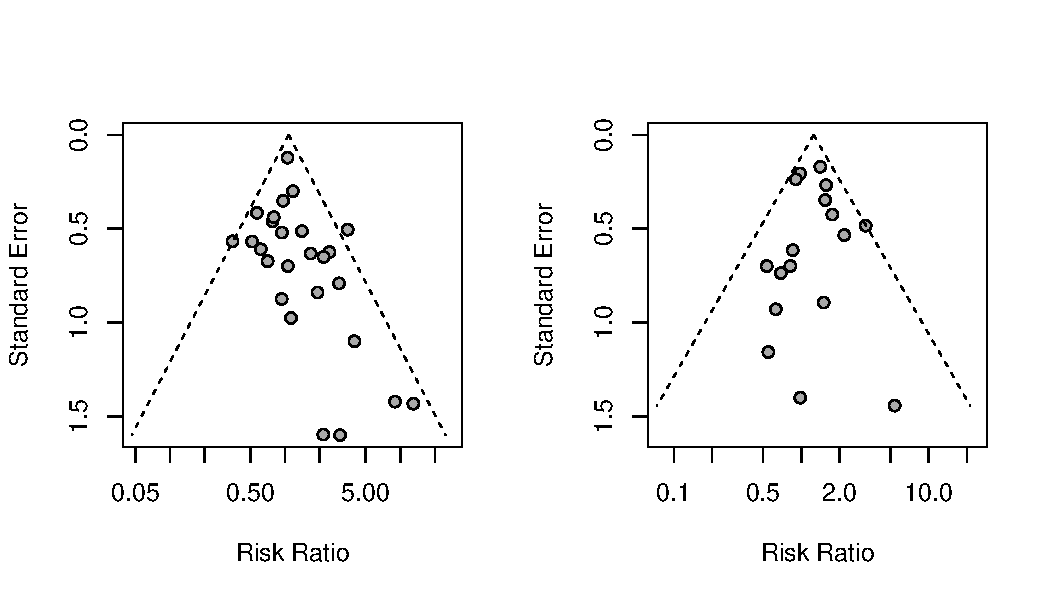
\includegraphics[width=\maxwidth]{figure/unnamed-chunk-2-1} 

\end{knitrout}
\end{figure}

\end{frame}


\begin{frame}[fragile]{Funnel Plot}
Effects with large standard errors have larger effect sizes (because they are only published
if significant)

\vspace{-10mm}
\begin{figure}
\begin{knitrout}
\definecolor{shadecolor}{rgb}{0.969, 0.969, 0.969}\color{fgcolor}
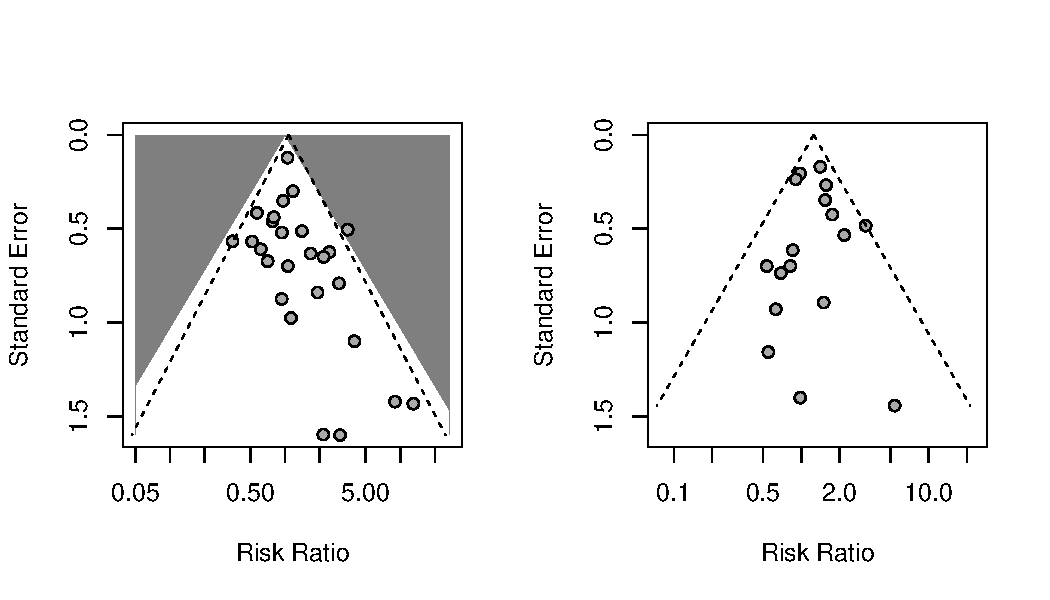
\includegraphics[width=\maxwidth]{figure/unnamed-chunk-3-1} 

\end{knitrout}
\end{figure}
\end{frame}

\begin{frame}{Detect Publication Bias}
\begin{itemize}
\item Small study effect tests (funnel plot asymmetry)
\item Excess significance tests
\end{itemize}
\end{frame}

\begin{frame}{Excess Significance Test}
Calculate power of each study, given that true effect size is
fixed effects meta-analysis estimate.

Calculate:
\begin{align}
p &= \sum_{i = O}^n\Big({n \choose i} p^i (1-p)^{n - i}\Big) \nonumber
\end{align}

\vspace{-1mm}
$O = $ observed no. of significant results, $E$ expected based on power of studies, $p$ = $E/n$.
\end{frame}

\begin{frame}{Analysis}
\begin{itemize}
\item Use meta-analyses from Cochrane.
\item ``The single most reliable source of evidence in clinical science
\end{itemize}

Analyse meta-analyses with publication bias tests.
\end{frame}

%------------------------------------------------------------------------------------------------%
\begin{frame}{The Cochrane Dataset}
\small
\begin{figure}
\begin{center}
\tikzstyle{block} = [rectangle, draw, fill=blue!20, text centered, rounded corners, minimum height=2.3em]
\tikzstyle{btw} = [rectangle, node distance=0cm, minimum height =1.8em, fill= white]
\tikzstyle{ublock} = [rectangle, draw, fill=blue!20, text centered, rounded corners, minimum height=4em, text width = 10em]
\tikzstyle{line} = [draw, ->, thick]
\tikzstyle{final} = [rectangle, draw, fill=red!20, text centered, rounded corners, minimum height=2.8em]

\begin{tikzpicture}[node distance = 2cm, auto]

        \node [final] (1) {Inital dataset:
    6,354 reviews,
    70,662 studies,
    744,720 results};
    
    \node [final, below of=1, node distance=2cm] (7) {Analysis dataset: 
    738 reviews,
    14,320 studies,
    22,937 results};

    \path [line] (1) -- node [btw, xshift = -2.8cm] {exclusion of unsuitable meta-analyses} (7);
\end{tikzpicture}
\label{Inclusion.criteria}
\end{center}
\end{figure}
\end{frame}

\begin{frame}{The Analysis dataset}
\footnotesize
\begin{figure}
\begin{center}
\tikzstyle{block} = [rectangle, draw, fill=blue!20, text centered, rounded corners, minimum height=2.3em]
\tikzstyle{btw} = [rectangle, node distance=0cm, minimum height =1.8em, fill= white]
\tikzstyle{ublock} = [rectangle, draw, fill=blue!20, text centered, rounded corners, minimum height=4em, text width = 10em]
\tikzstyle{line} = [draw, ->, thick]
\tikzstyle{final} = [rectangle, draw, fill=red!20, text centered, rounded corners, minimum height=2.8em]

\begin{tikzpicture}[node distance = 2cm, auto]


    \node [final, node distance=1cm] (7) {Analysis dataset:
    1,388 meta-analyses};


    \node [ublock, below of=7, node distance=3.5cm] (8) {Binary data: \\
    924 meta-analyses};

    \node [ublock, right of=8, node distance=3.5cm] (9) {Continuous data: \\
    343 meta-analyses};

    \node [ublock, left of=8, node distance=3.5cm] (10) {Other data (IV): \\
    121 meta-analyses};


    \path [line] (7) -- (8);
    \path [line] (7) --  (9);
    \path [line] (7) --  (10);
    
\end{tikzpicture}

\end{center}
\end{figure}
\end{frame}


\begin{frame}{Small Study Effect Tests}
\vspace{-4mm}
Weighted linear regression with std. error $x_i$ and effect size $y_i$:
\begin{align}
y_i &= \beta_0 + \beta_1 x_i + \epsilon_i, & \epsilon_i \sim N(0, x_i \sigma^2) \nonumber
\end{align}
Test for $H0: \beta_1 = 0$, no funnel plot asymmetry
\end{frame}

\begin{frame}{Adjustments for Binary Data}
As recommended by \citet{Sterne}
\begin{itemize}
\item Log odds ratio and risk ratio $\theta$ and standard error $\se_\theta$ are not independent
\item Use score of binomial likelihood at log odds ratio $\theta_{\textrm{H0}} = 0$ instead of 
log odds ratio, and the inverse Fisher information instead of $\se_\theta$
\end{itemize}
\end{frame}


\begin{frame}[fragile]{Small Study Effect Tests}
\begin{figure}
\begin{knitrout}
\definecolor{shadecolor}{rgb}{0.969, 0.969, 0.969}\color{fgcolor}
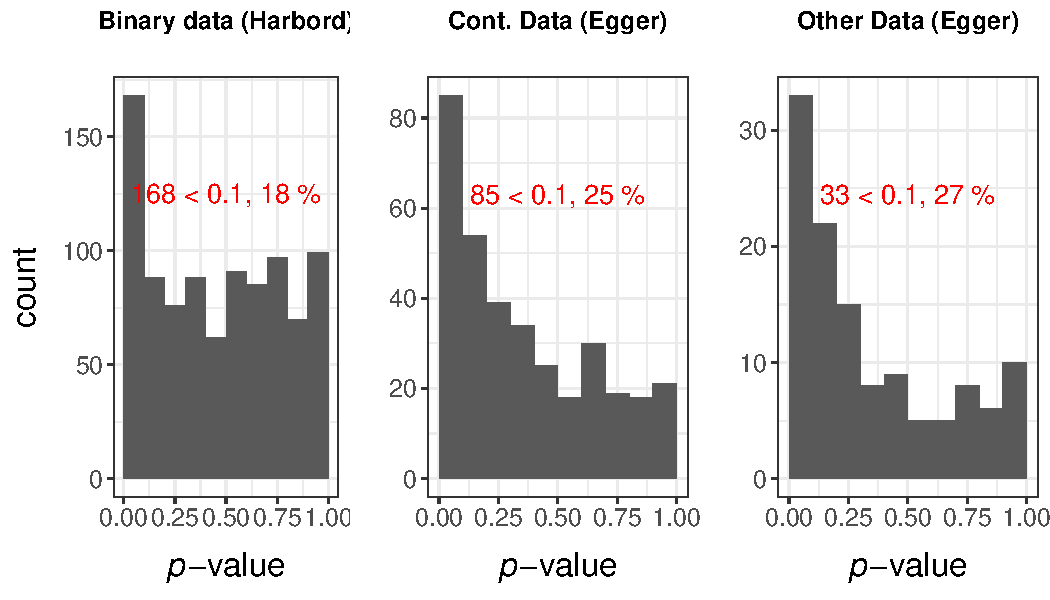
\includegraphics[width=\maxwidth]{figure/unnamed-chunk-4-1} 

\end{knitrout}
\end{figure}
\end{frame}


\begin{frame}[fragile]{Excess Significance Test}
\begin{figure}
\begin{knitrout}
\definecolor{shadecolor}{rgb}{0.969, 0.969, 0.969}\color{fgcolor}
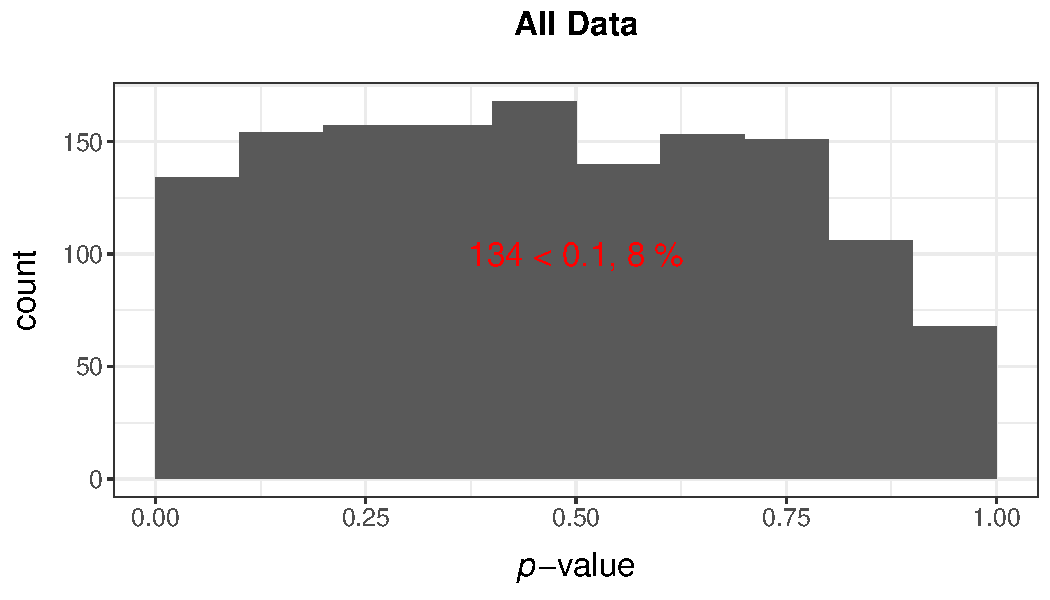
\includegraphics[width=\maxwidth]{figure/unnamed-chunk-5-1} 

\end{knitrout}
\end{figure}
\end{frame}

\begin{frame}{Adjustment}
Calculate unbiased estimates by
\begin{itemize}
\item Sensitivity analysis
\item Regression approach
\end{itemize}
\end{frame}

\begin{frame}{Selection Model}
\citet{Copas2}
\begin{align}
\theta_i &\sim N(\mu_i, \sigma_i^2) &
\mu_i \sim N(\theta, \tau^2) \nonumber
\end{align}
So we have $\theta_i = \mu_i + \sigma_i\epsilon_i \nonumber$. Introduce
\begin{itemize}
\item Baseline study retention rate $a$
\item Std. error dependent retention rate $b$
\item introduces correlation between $\epsilon_i$ and selection probability
\end{itemize}
%Model the selection process for increasing $a$ and $b$
\end{frame}

\begin{frame}{Sensitivity analysis}
To test a pair $a$,$b$,	include $\beta$:
\begin{align}
\theta_i &= \theta + \beta \se_i + \sigma_i \epsilon_i \nonumber
\end{align}
\vspace{-10mm}
\begin{itemize}
\item $\theta_i$ is the effect size of study $i$ and right-hand side is the fitted 
value of the model. 
\item Repeatedly test for $\beta_{\textrm{H0}} = 0$ %and estimate $\theta_{\textrm{Adj.}}$
\end{itemize}
\end{frame}

\begin{frame}{Regression}
Correct for small study effect \citep{Limitmeta}:
\begin{itemize}
\item Use global mean of regression $\beta_0$ from $y_i = \beta_0 + \beta_1 x_i + \epsilon_i, \epsilon_i \sim N(0, x_i \sigma^2) \nonumber$
\item Add minimal bias term $\beta_1 \cdot \tau$
\end{itemize}
$\theta_{\textrm{Adj.}} = \beta_0 + \beta_1\tau$
\end{frame}

\begin{frame}{Adjustment Methods}
Differences:
\begin{itemize}
\item Regression: uncertainty of bias parameter retained
\item Sensitivity analysis: Bias itself is not estimated, but most parsimonious scenario is chosen
\item Sensitivity analysis: No adjustment if no evidence for bias
\end{itemize}
Regression adjustment leads to higher uncertainty of $\theta_{\textrm{Adj.}}$
\end{frame}

\begin{frame}{Effect Measure Transformation}
\vspace{-3mm}
\begin{align}
d &= \theta \frac{\sqrt{3}}{\pi} & \se_d^2 =  \se^2\frac{\sqrt{3}}{\pi} \nonumber
\end{align}
\begin{align}
r &= \frac{d}{\sqrt{d^2 + a}} & a = (n_c + n_t)^2 / n_c n_t \nonumber
\end{align}
\begin{align}
z &= 0.5 \ln\bigg(\frac{1 + r}{1 - r}\bigg) & \nonumber
%z &= \arctan(r) & \nonumber
\se_z^2 &= \frac{1}{n-3}
\end{align}
\end{frame}

\begin{frame}[fragile]{Results}
\begin{knitrout}
\definecolor{shadecolor}{rgb}{0.969, 0.969, 0.969}\color{fgcolor}
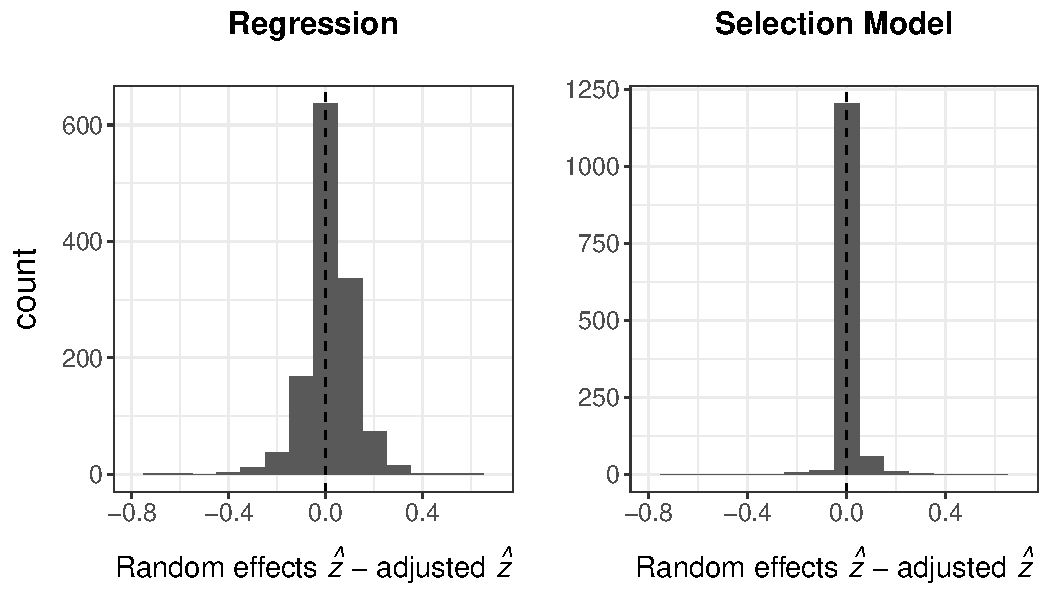
\includegraphics[width=\maxwidth]{figure/unnamed-chunk-6-1} 

\end{knitrout}
\end{frame}


\begin{frame}{Results}
% \vspace{-3mm}
% Compare wald test statistics (original effect size measures):
% 
% \vspace{-2mm}
\begin{knitrout}
\definecolor{shadecolor}{rgb}{0.969, 0.969, 0.969}\color{fgcolor}
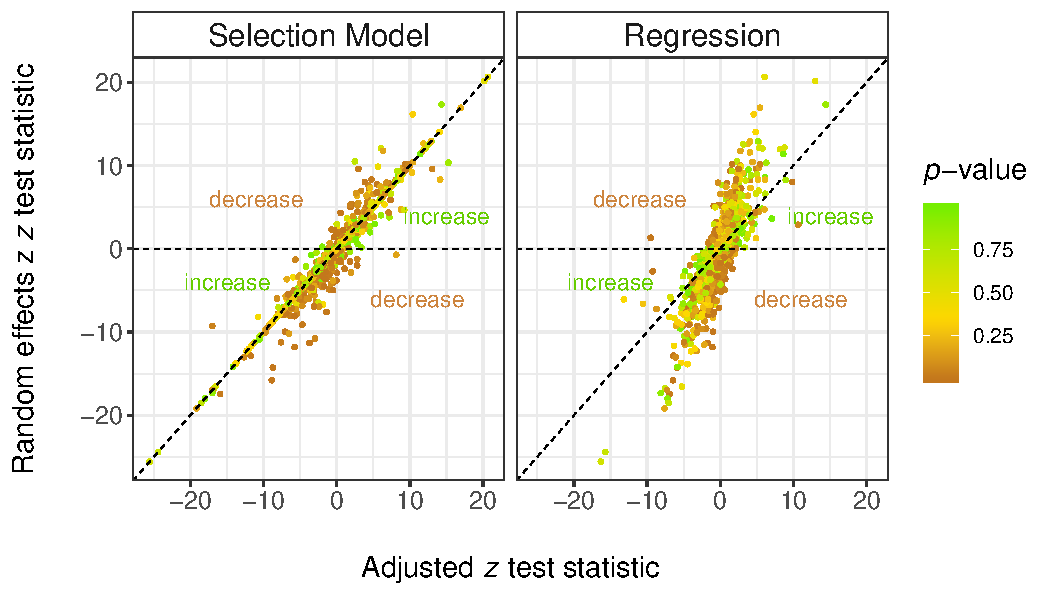
\includegraphics[width=\maxwidth]{figure/unnamed-chunk-7-1} 

\end{knitrout}

\end{frame}

\begin{frame}{Missing Study Number}
Missing study number according to selection model parameters: 2,618, 11.4\%


% latex table generated in R 3.5.1 by xtable 1.8-3 package
% Wed Aug 21 13:58:04 2019
\begin{table}[ht]
\centering
\begingroup\footnotesize
\begin{tabular}{lrrrrrrr}
  \hline
 & = 0 & 5\% & 25\% & 50\% & 75\% & 95\% & mean \\ 
  \hline
Missing number & 226 & 0 & 0 & 1.5 & 5.9 & 20.1 & 4.7 \\ 
  Overall fraction & 226 & 0 & 0 & 0.1 & 0.4 & 1.0 & 0.3 \\ 
   \hline
\end{tabular}
\endgroup
\caption{Fraction of missing studies and estimates of missing studies with their zero counts (``= 0''), quantiles and means.} 
\label{copas.missing}
\end{table}

\end{frame}

\begin{frame}{Additional Results}
Linear mixed model with random effects for meta-analyses and reviews:

\begin{align}
\mathbf{y}_i \given U_j,U_k,\epsilon_{i} =  \beta_0 + x_i\beta_1 + U_j + U_k + \epsilon_{i} \nonumber
\end{align}

$\rightarrow$ Increased power to estimate $\beta$
\end{frame}

\begin{frame}{Mixed Linear Model}
AIC improvement to null fit: 1820 to 1306. \\
Bias parameter $\beta_1$ = 0.52 (95\%CI: 0.44,0.59)

\vspace{-12mm}
\begin{figure}
\begin{knitrout}
\definecolor{shadecolor}{rgb}{0.969, 0.969, 0.969}\color{fgcolor}
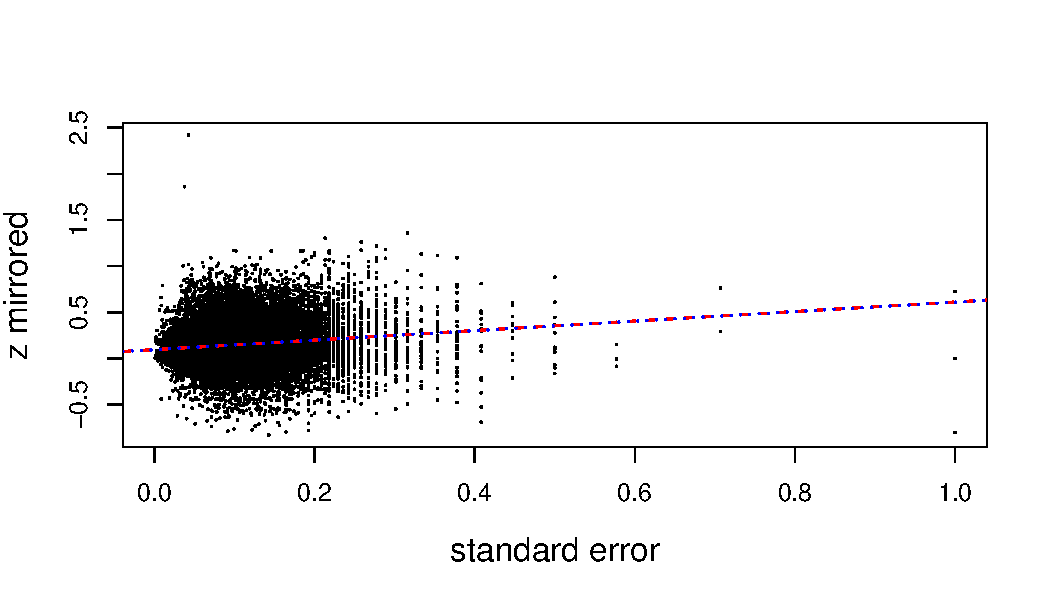
\includegraphics[width=\maxwidth]{figure/unnamed-chunk-9-1} 

\end{knitrout}
\end{figure}
\end{frame}

\begin{frame}{Limitations}
Small study effect $\neq$ publication bias. Also:
\begin{itemize}
\item True heterogeneity
\item Selective outcome reporting
\item Delayed publication
\item ...
\end{itemize}
\vspace{-3mm}
Small study effect tests do not take into account significance directly.
\end{frame}

\begin{frame}{Limitations}
\begin{itemize}
\item Unknown amount of secondary outcomes
\item Small amount of adverse outcomes
\item Publication bias unknown for excluded data
\item Exploratory Analysis!
\end{itemize}
\end{frame}

\begin{frame}{Implications}
\begin{itemize}
\item Results are largely in line with previous research
\item Underline the need for examination of publication and other biases in meta-analyses
\item Otherwise, validity of meta-analyses can be contested
\end{itemize}
\end{frame}


\begin{frame}{References}
  \small
  \bibliographystyle{apalike}
\bibliography{illustration}
\end{frame}


\begin{frame}
Backup slides:
\end{frame}

\begin{frame}[fragile]{Transformation}

\vspace{-6mm}
\begin{knitrout}
\definecolor{shadecolor}{rgb}{0.969, 0.969, 0.969}\color{fgcolor}
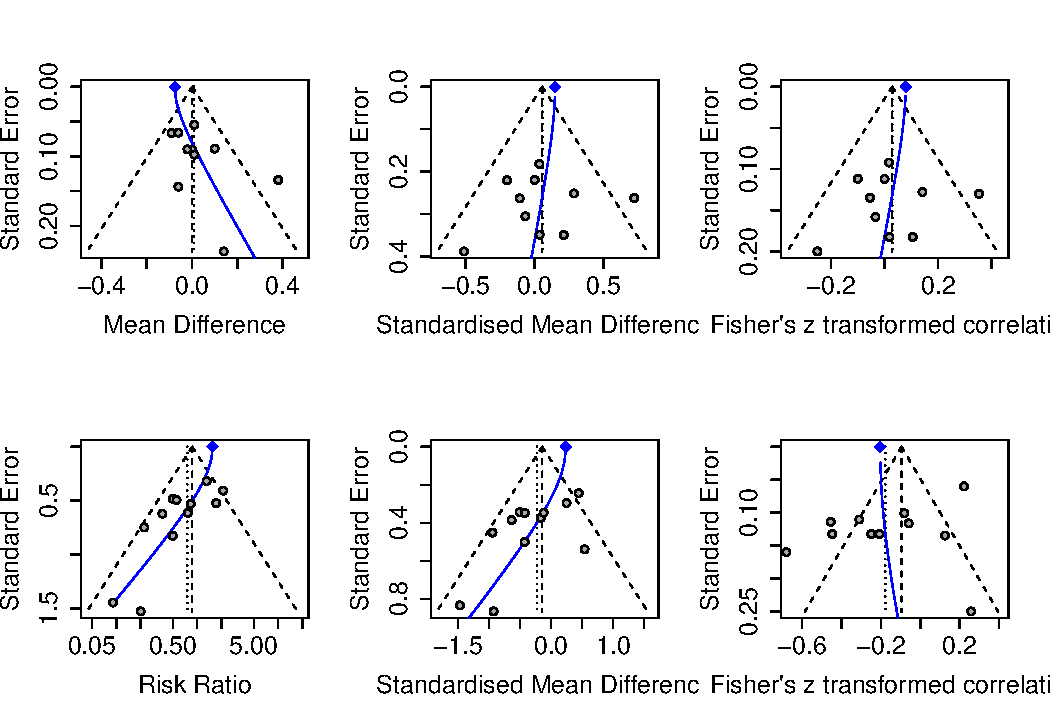
\includegraphics[width=\maxwidth]{figure/unnamed-chunk-10-1} 

\end{knitrout}
\end{frame}


















% 
% \begin{frame}{Fixed Effects Meta-Analysis}
% Study $i$ of $n$ studies, effects $\theta_i$ and variances $v_i$, s.e. $s_i$
% 
% Fixed effects estimate: weighted mean with $w_i = 1/\hat{v_i}$: 
% 
% \begin{align}
% \theta_f &= \frac{\sum_{i = 1}^n w_{i}\theta_i}{\sum_{i = 1}^n w_i} \nonumber \\ 
% \textrm{se}(\theta_f) &= \frac{1}{\sqrt{\sum_{i = 1}^n w_i}} \nonumber
% \end{align}
% \end{frame}
% 
% \begin{frame}{Random Effects Meta-Analysis}
% Let $\hat{\theta_i}|\theta_i \sim N(\theta_i, v_i) 
% \theta_i \sim N(\theta, \tau^2)$
% 
% Random effects estimate: weigthed mean of $\hat{\theta_i}$ with weights $w_i = 1/(\hat{v_i} + \tau^2)$
% \end{frame}
% 
% \begin{frame}{Evidence Based Medicine}
% Likely to base decisions on over-optimistic findings
% 
% Direct consequences: patient harm and unnecessary research
% \end{frame}
% 
% 
% \begin{frame}{Cochrane Organisation}
% Aim: summarise findings in primary clinical research and health care
% 
% Provide peer-reviewed, systematic reviews
% 
% Public access (for some countries)
% \end{frame}
% 
% \begin{frame}{Research Question}
% Quantify the abundance and impact of publication bias in the Cochrane Library
% \end{frame}
% 
% 
% \begin{frame}{Cochrane Library Dataset}
% format(length(unique(data$file.nr)), big.mark=",") systematic reviews with studies published until 2018.
% 
% format(length(unique(data$study.name)), big.mark=",") studies.
% 
% format(dim(data)[1], big.mark=",") study results.
% \end{frame}
% 
% 
% \begin{frame}[fragile]{Review Example: Binary Outcome}
% Barbiturate efficacy for head injury treatment
% \vspace{-5mm}
% <<echo = FALSE, results = 'asis'>>=
% print(xtable(barbi2, label = "barbiturates", digits = 0), include.rownames = F, size = "tiny")
% @
% \end{frame}
% 
% 
% 
% \begin{frame}{Dataset Structure}
% 
% \begin{figure}
% \tikzstyle{every node}=[draw=black,thick,anchor=west,scale=.65]
% \tikzstyle{selected}=[draw=red,fill=red!30]
% \tikzstyle{optional}=[dashed,fill=gray!50]
% \begin{tikzpicture}
% [grow = right, anchor = west,
%   growth parent anchor=east, % added code
%   parent anchor=east, level distance=.5cm,
%   sibling distance=2em, level 1/.style={sibling distance=2em}, level 2/.style={sibling distance=2em},
%   level 3/.style={sibling distance=2em}, level 4/.style={sibling distance=1.2em}]
%   \node {Review} [edge from parent fork right]
%     child { node {Comparison 2}
%       child { node {Outcome 2}}
%       child { node {Outcome 1}
%         child { node {Subgroup 2}}
%         child { node {Subgroup 1}
%           child  { node {Result 3}}
%           child  { node {Result 2}}
%           child  { node {Result 1}}
%           }}
%     }
%     child [missing] {}
%     child { node {Comparison 1}};
% \end{tikzpicture}
% %\caption{Structure of a hypothetical review with two different comparisons\label{review.structure}}
% \label{review.structure}
% \end{figure}
% \end{frame}
% 
% 
% 
% 
% 
% \begin{frame}[fragile]{Dataset Properties}
% Review or study level:
% <<echo=FALSE, results = 'asis'>>=
% print(xtable(dataset.properties, digits = 0, align = "lrrrr"), include.rownames = T, size = "footnotesize", hline = c(0,1,1,3))
% @
% \end{frame}
% 
% 
% 
% \begin{frame}{Small Study Effects}
% ``The tendency for the smaller studies to show larger treatment effects'' \citep{Sterne}
% \end{frame}
% 
% 
% \begin{frame}{Small Study Effects}
% Causes:
% \begin{itemize}
% \item Selective publication of studies with significant results - publication bias
% \item Systematic differences in study settings
% \end{itemize}
% \end{frame}
% 
% 
% \begin{frame}{Small Study Effect Tests}
% Different approaches:
% \begin{itemize}
% \item Simple linear regression
% \item Rank correlation
% \end{itemize}
% 
% Special methods for binary outcomes	
% \end{frame}
% 
% 
% % \begin{frame}[fragile]{Small Study Effect Tests}
% % Funnel plots (continuous outcome examples):
% % 
% % \vspace{-1.2cm}
% % 
% % <<message = FALSE, echo=FALSE, warning = FALSE, fig.height=4>>=
% % par(las = 1, mfrow = c(1, 2))
% % funnel(meta.example)
% % funnel(meta.nexample)
% % @
% % 
% % \end{frame}
% % 
% % 
% % \begin{frame}[fragile]{Regression based Tests}
% % Radial plots (continuous outcome examples):
% % 
% % \vspace{-1.1cm}
% % 
% % <<message = FALSE, echo=FALSE, warning = FALSE, fig.height=4>>=
% % par(las = 1, mfrow = c(1,2))
% % biased.rev$inv <- 1/biased.rev$se
% % plot(y = (biased.rev$effect/biased.rev$se), x = (biased.rev$se^-1), xlim = c(0, 6), xlab = "inverse standard error", 
% % 		 ylab = "mean diff. / std. error")
% % 
% % unbiased.rev$inv <- 1/unbiased.rev$se
% % plot(y = (unbiased.rev$effect/unbiased.rev$se), x = (unbiased.rev$inv), xlim = c(0, 1.2), 
% % 		 ylim = c(-18, 0), xlab = "inverse standard error", ylab = "mean diff. / std. error")
% % @
% % 
% % \end{frame}
% 
% 
% \begin{frame}{Regression based Tests}
% study $i$ of $n$ studies, effects $\theta_i$ and variances $v_i$, s.e. $s_i$
% 
% $\theta_M$ is the pooled effect and $\tau^2$ the between-study variance.
% 
% Let $y_{i} = \theta_{i}/_{i}$ and $x_i = 1/s_i$
% \begin{itemize}
% \item \citet{Egger} : Simple linear regression \\ $y_i = \beta_0 + \beta_1 x_i, \epsilon_i \sim N(0, \sigma)$
% \item \citet{thompson.sharp} : extension of Egger with study weights $v_{i} + \tau^2$ 
% \end{itemize}
% 
% \end{frame}
% 
% \begin{frame}[fragile]{Egger's Test examples}
% Test for non-zero intercept $\beta_{0}$
% 
% \vspace{-1.1cm}
% <<message = FALSE, echo=FALSE, warning = FALSE, fig.height=4>>=
% par(las = 1, mfrow = c(1,2))
% biased.rev$inv <- 1/biased.rev$se
% m.ex <- lm(formula = (biased.rev$effect/biased.rev$se) ~ (biased.rev$inv))
% plot(y = (biased.rev$effect/biased.rev$se), x = (biased.rev$se^-1), xlim = c(0, 6), xlab = "inverse standard error", 
% 		 ylab = "mean diff. / std. error")
% abline(coef = coef(m.ex), lty = 2, col = 2)
% 
% 
% unbiased.rev$inv <- 1/unbiased.rev$se
% m.nex <- lm(formula = (unbiased.rev$effect/unbiased.rev$se) ~ (unbiased.rev$inv))
% plot(y = (unbiased.rev$effect/unbiased.rev$se), x = (unbiased.rev$inv), xlim = c(0, 1.2), 
% 		 ylim = c(-18, 0), xlab = "inverse standard error", ylab = "mean diff. / std. error")
% abline(coef = coef(m.nex), lty = 2, col = 2)
% @
% \end{frame}
% 
% 
% \begin{frame}{Regression Tests for Binary Outcomes}
% 
% \begin{itemize}
% \item \citet{Peters} :$x_i = 1/n_i$ instead $1/s_i$, inverse variances as weight.
% \item \citet{Harbord} :$x_i$ = score of the log-likelihood of a proportion and inverse variances as weights.
% \item \citet{Rucker} :Use arcsine variance stabilizing transformation for variances and effects, do e.g. Egger's test.
% \end{itemize}
% \end{frame}
% 
% 
% \begin{frame}{Rank based tests}
% \citet{begg.ties}: \\
% Let $y_{i}$ be $\frac{\theta_i - \theta_M}{v_i}$ and $x_i$ its variance ($\neq v_i$)
% 
% $u$ the number of pairs $(y_{i}, x_{i})$ ranked in the same order, $l$
% the number of pairs in the opposite order
% 
% $Z = \frac{(u - l)}{\sqrt{n(n-1)(2n + 5)/18}}$  is a test statistic
% \end{frame}
% 
% \begin{frame}{Rank based tests}
% \citet{Schwarzer}: \\
% $e_t$ number of events in the treatment group
% 
% $E_t$ follows hypergeometric distribution: calculate $\mathbb{E}(E_{t})$ and variances
% 
% proceed as in \citet{begg.ties}
% \end{frame}
% 
% 
% \begin{frame}{Test Results}
% Inclusion criteria (from \citet{Ioannidis2007}):
% \begin{itemize}
% \item $n \geq 10$
% \item at least one statistically significant effect in a study
% \item $\frac{\hat{v_{\textrm{max}}}^2}{\hat{v_{\textrm{min}}}^2} > 4$
% \item $I^2 < 0.5$
% \end{itemize}
% 
% From dim(meta)[1] with $n \geq 10$, dim(meta.f)[1] remain.
% \end{frame}
% 
% 
% 
% \begin{frame}[fragile]{Continuous Outcome Test Results}
% $p$-values distribution, $n$ = dim(meta.cont)[1]:
% 
% \vspace{-2mm}
% <<echo = FALSE, fig.height = 4, message = FALSE>>=
% plot(p.dist.cont)
% @
% \end{frame}
% 
% \begin{frame}[fragile]{Binary Outcome Test Results}
% $p$-values distribution, $n$ = dim(meta.bin)[1]:
% 
% \vspace{-2mm}
% <<echo = FALSE, fig.height = 3.6, message = FALSE>>=
% plot(p.dist.bin)
% @
% \end{frame}
% 
% \begin{frame}[fragile]{Agreement in significance}
% Number of significant test results per meta-analysis:
% 
% \vspace{-2mm}
% <<echo = FALSE, fig.height = 3.2, message = FALSE>>=
% grid.arrange(agree.cont, agree.bin, ncol = 2)
% @
% \end{frame}
% 
% \begin{frame}{Small Study Effect Adjustment}
% Three methods:
% \begin{itemize}
% \item Regression
% \item Copas selection model
% \item Trim-and-fill
% \end{itemize}
% \end{frame}
% 
% \begin{frame}{Adjustment by regression}
% $y_i = \theta_i/s_i, x_i = 1/s_i$
% 
% $y_i = \beta_0 + \beta_1 x_i, \epsilon_i \sim N(0, \sigma)$
% 
% $\beta_1$ is the weighted mean treatment effect if $\beta_0 = 0$
% \end{frame}
% 
% 
% \begin{frame}{Adjustment by regression}
% Radial plots (continuous outcome examples):
% 
% \vspace{-1.1cm}
% 
% <<message = FALSE, echo=FALSE, warning = FALSE, fig.height=4>>=
% par(las = 1, mfrow = c(1,2))
% biased.rev$inv <- 1/biased.rev$se
% m.ex.0 <- lm(formula = (biased.rev$effect/biased.rev$se) ~ 0 + (biased.rev$inv))
% m.ex <- lm(formula = (biased.rev$effect/biased.rev$se) ~ (biased.rev$inv))
% plot(y = (biased.rev$effect/biased.rev$se), x = (biased.rev$se^-1), xlim = c(0, 6), xlab = "inverse standard error", 
% 		 ylab = "mean diff. / std. error")
% abline(coef = c(0,coef(m.ex.0)), lty = 2)
% abline(coef = coef(m.ex), lty = 2, col = 2)
% 
% 
% unbiased.rev$inv <- 1/unbiased.rev$se
% m.nex.0 <- lm(formula = (unbiased.rev$effect/unbiased.rev$se) ~ 0 + (unbiased.rev$inv))
% m.nex <- lm(formula = (unbiased.rev$effect/unbiased.rev$se) ~ (unbiased.rev$inv))
% plot(y = (unbiased.rev$effect/unbiased.rev$se), x = (unbiased.rev$inv), xlim = c(0, 1), 
% 		 ylim = c(-18, 0), xlab = "inverse standard error", ylab = "mean diff. / std. error")
% abline(coef = c(0,coef(m.nex.0)), lty = 2)
% abline(coef = coef(m.nex), lty = 2, col = 2)
% @
% \end{frame}
% 
% 
% 
% \begin{frame}[fragile]{Limit Meta-Analysis}
% Extended random effects model:
% 
% \vspace{-4mm}
% \begin{align}
% \theta_i = \beta_0 + \beta_1(\sqrt{v_i + \tau^2}) + \epsilon_i(\sqrt{v_i + \tau^2}), \nonumber \\
% \epsilon_{i} \stackrel{\textrm{iid}}{\sim} N(0,1) \nonumber
% \end{align}
% 
% Use $\mathbb{E}(\theta_{i}) \rightarrow \beta_{0} + \beta_{1}\tau$ for $\sqrt{v_{i}} \rightarrow 0$
% as corrected treatment efffect.
% \end{frame}
% 
% 
% 
% \begin{frame}[fragile]{Limit Meta-Analysis}
% Funnel plot with effect with infinite precision:
% 
% \vspace{-1.1cm}
% <<message = FALSE, echo=FALSE, warning = FALSE, fig.height=4>>=
% par(las = 1, mfrow = c(1,2))
% funnel(limitmeta(meta.example))
% funnel(limitmeta(meta.nexample))
% @
% \end{frame}
% 
% 
% 
% \begin{frame}{Selection model}
% \citet{Copas1}: model based on a bivariate normal distribution:
% 
% \vspace{-8mm}
% \begin{align}
% \hat{\theta_i} = \theta_{i} + \sigma_i\epsilon_i \label{population.model2} \\
% \theta_i \sim N(\theta, \tau^2) \label{population.model} \\
% z_i = a + b/\hat{s_i} + \delta_i \label{selection.model}
% \end{align}
% 
% \ref{population.model2},\ref{population.model} is called population model, \ref{selection.model} the selection model
% 
% $(\epsilon_i, \delta_i)$ are standard normal residuals with correlation $\rho = cor(y_i, z_i)$.
% \end{frame}
% 
% 
% \begin{frame}[fragile]{Sensitivity Analysis}
% Model the selection process with different $a,b$
% 
% Test if small study effect is significant, by including \\ $\theta_i = \theta_i + \beta s_i + v_{i}\epsilon_i$
% 
% Estimation: Select $a, b$ such that $H0$ can not be rejected and estimated
% number of unpublished studies is minimal.
% \end{frame}
% 
% 
% \begin{frame}{Trim-and-Fill}
% Mirror studies that cause asymmetry:
% \vspace{-1.2cm}
% 
% <<message = FALSE, echo=FALSE, warning = FALSE, fig.height=4>>=
% par(las = 1, mfrow = c(1, 2))
% funnel(meta.example)
% funnel(meta.nexample)
% @
% \end{frame}
% 
% 
% \begin{frame}[fragile]{Results:}
% Difference between random and fixed effects meta-analysis estimate: $|\theta_f - \theta_{r}|$
% 
% \vspace{-3mm}
% <<echo = FALSE, fig.height = 3.6, message = FALSE, warning=FALSE>>=
% plot(hist.ranef)
% @
% \end{frame}
% 
% 
% \begin{frame}[fragile]{Adjustment Results: Trim-and-fill}
% Absolute difference between adjusted and fixed effects meta-analysis estimate: $|{\theta_f} - {\theta_{\textrm{adjusted}}}|$
% 
% \vspace{-3mm}
% <<echo = FALSE, fig.height = 3.6, message = FALSE, warning=FALSE>>=
% plot(hist.trimfill1)
% @
% \end{frame}
% 
% 
% \begin{frame}[fragile]{Adjustment Results: Copas}
% Absolute difference between adjusted and fixed effects meta-analysis estimate: $|{\theta_f} - {\theta_{\textrm{adjusted}}}|$
% 
% \vspace{-3mm}
% <<echo = FALSE, fig.height = 3.6, message = FALSE, warning=FALSE>>=
% plot(hist.copas1)
% @
% \end{frame}
% 
% 
% \begin{frame}[fragile]{Adjustment Results: Regression}
% Absolute difference between adjusted and fixed effects meta-analysis estimate: $|{\theta_f} - {\theta_{\textrm{adjusted}}}|$
% 
% \vspace{-3mm}
% <<echo = FALSE, fig.height = 3.6, message = FALSE, warning=FALSE>>=
% plot(hist.reg1)
% @
% \end{frame}
% 
% 
% \begin{frame}[fragile]{Results:}
% Random and fixed effects meta-analyses test statistics:
% 
% \vspace{-3mm} 
% <<echo = FALSE, fig.height = 3.8, message = FALSE, warning=FALSE>>=
% plot(ranef.fixef.sc.zval)
% @
% \end{frame}
% 
% 
% \begin{frame}[fragile]{Adjustment Results: Trim-and-fill}
% Adjusted and meta-analysis test statistics:
% 
% \vspace{-3mm} 
% <<echo = FALSE, fig.height = 3.8, message = FALSE, warning=FALSE>>=
% grid.arrange(trimfill.fixef.sc.zval, trimfill.ranef.sc.zval, ncol = 2)
% @
% \end{frame}
% 
% 
% \begin{frame}[fragile]{Adjustment Results: Copas}
% Adjusted and meta-analysis test statistics:
% 
% \vspace{-3mm}
% <<echo = FALSE, fig.height = 3.8, message = FALSE, warning=FALSE>>=
% grid.arrange(copas.fixef.sc.zval, copas.ranef.sc.zval, ncol = 2)
% @
% \end{frame}
% 
% 
% \begin{frame}[fragile]{Adjustment Results: Regression}
% Adjusted and meta-analysis test statistics:
% 
% \vspace{-3mm}
% <<echo = FALSE, fig.height = 3.8, message = FALSE, warning=FALSE>>=
% grid.arrange(reg.fixef.sc.zval, reg.ranef.sc.zval, ncol = 2)
% @
% \end{frame}
% 
% 
% \begin{frame}[fragile]{Adjustment Results}
% Missing study proportions:
% 
% \vspace{-3mm}
% <<echo = FALSE, fig.height = 3.8, message = FALSE, warning=FALSE>>=
% grid.arrange(p.missing.copas, p.missing.trim, ncol = 2) 
% @
% \end{frame}
% 
% \begin{frame}[fragile]{Extreme Results}
% RR reduction by trimfill (-3.9), side effects
% 
% <<echo = FALSE, fig.height = 3.5>>=
% trimfill.id(165815)
% @
% \end{frame}
% 
% \begin{frame}[fragile]{Extreme Results}
% RR Reduction by copas selection model (-4), pain relief
% 
% <<echo = FALSE, fig.height = 3.5>>=
% funnel.id(73169)
% @
% \end{frame}
% 
% \begin{frame}[fragile]{Extreme Results}
% RR Amplification by regression (+14), side effects
% 
% <<echo = FALSE, fig.height = 3.5, warning=FALSE>>=
% limitmeta.id(119537)
% @
% \end{frame}
% 
% \begin{frame}[fragile]{Discussion}
% \begin{itemize}
% \item Proportion of positive tests is well above 10\%
% \item Effect sizes and evidence for treatment effect is diminishued
% \item Limitations: not only primary outcomes, adjustment methods known to
% perform poorly under the 0
% \end{itemize}
% \end{frame}
% 
% 
% \begin{frame}[fragile]{Outlook}
% \begin{itemize}
% \item Connect results with different medical fields, look for differences
% \item Connect results with single studies and journals (?)
% \end{itemize}
% \end{frame}
% 
% 
% 
% 
% 
% 
% 
% 
% 
% 
% 
% 
% 
% %%%%%%%%%%%%%%%%%%%%%%%%%%%%%%%%%%%%%%%%%%%%%%%%%%%%%%%%%%%%%%%%%%%%%%%%
% %Backup Slides%%%%%%%%%%%%%%%%%%%%%%%%%%%%%%%%%%%%%%%%%%%%%%%%%%%%%%%%%%
% %%%%%%%%%%%%%%%%%%%%%%%%%%%%%%%%%%%%%%%%%%%%%%%%%%%%%%%%%%%%%%%%%%%%%%%%
% 
% \begin{frame}[fragile]{Adjustment Results: Trim-and-fill}
% Treatment effect difference:
% 
% \vspace{-3mm}
% <<echo = FALSE, fig.height = 4, message = FALSE, warning=FALSE>>=
% plot(hist.trimfill)
% @
% \end{frame}
% 
% 
% \begin{frame}[fragile]{Adjustment Results: Copas}
% Treatment effect difference:
% 
% \vspace{-3mm}
% <<echo = FALSE, fig.height = 4, message = FALSE, warning=FALSE>>=
% plot(hist.copas)
% @
% \end{frame}
% 
% 
% \begin{frame}[fragile]{Adjustment Results: Regression}
% Treatment effect difference:
% 
% \vspace{-3mm}
% <<echo = FALSE, fig.height = 4, message = FALSE, warning=FALSE>>=
% plot(hist.reg)
% @
% \end{frame}
% 
% \begin{frame}[fragile]{Results}
% log treatment effect estimates:
% 
% \vspace{-3mm}
% <<echo = FALSE, fig.height = 4, message = FALSE, warning=FALSE>>=
% plot(ranef.fixef.sc.effect)
% @
% \end{frame}
% 
% \begin{frame}[fragile]{Adjustment Results: Trim-and-fill}
% log treatment effect estimates:
% 
% \vspace{-3mm}
% <<echo = FALSE, fig.height = 4, message = FALSE, warning=FALSE>>=
% grid.arrange(trimfill.fixef.sc.effect, trimfill.ranef.sc.effect, ncol = 2)
% @
% \end{frame}
% 
% 
% \begin{frame}[fragile]{Adjustment Results: Copas}
% log treatment effect estimates:
% 
% \vspace{-3mm}
% <<echo = FALSE, fig.height = 4, message = FALSE, warning=FALSE>>=
% grid.arrange(copas.fixef.sc.effect, copas.ranef.sc.effect, ncol = 2)
% @
% \end{frame}
% 
% 
% \begin{frame}[fragile]{Adjustment Results: Regression}
% log treatment effect estimates:
% 
% \vspace{-3mm}
% <<echo = FALSE, fig.height = 4, message = FALSE, warning=FALSE>>=
% grid.arrange(reg.fixef.sc.effect, reg.ranef.sc.effect, ncol = 2)
% @
% \end{frame}
% 
% 
% 
% 




%\appendix
%% Possible backup slides...

%% chapter division is accomplished with:
%% \part{Appendix}

% \begin{frame}[fragile]{Test Results: Significance}
% 
% <<echo = FALSE, fig.height = 4>>=
% grid.arrange(p.bin, p.cont, ncol = 2)
% @
% \end{frame}

% \begin{frame}[fragile]{Pooling Studies - Meta-Analysis}
% Multiple results in a meta-analysis group can be pooled:
% <<echo=FALSE, results = 'asis'>>=
% print(xtable(cum.repr.trials.subg, label = "repr.groups", align = "lrrr", digits = 0), include.rownames = F, size = "footnotesize")
% @
% \end{frame}

% \begin{frame}{Dataset Structure}
% \begin{itemize}
% \item Comparison: What is compared, e.g. treatment vs. control
% \item Outcome: How it is compared
% \item Subgroup: Subgroup affiliation
% \item Meta-Analysis Group: Results from same comparison, outcome and subgroup
% \end{itemize}
% \end{frame}

% \begin{frame}[fragile]{Dataset Properties}
% Missing data:
% <<echo=FALSE, results = 'asis'>>=
% print(xtable(missing.table, align = "lr"), include.rownames = T, include.colnames = F)
% @
% \end{frame}




% \begin{frame}{Adjustment by regression}
% Similar to the tests, but with unnormalized effect $y_{i}$:
% 
% \begin{align}
% y_{i} = \beta_{0} + \beta_{1}x_{i}
% \end{align}
% 
% $\beta_{0}$	 corresponds to $y_{i}$ with $x_{i} = 0$
% \end{frame}
% 
% \begin{frame}[fragile]{Adjustment by regression}
% Linear regression method:
% 
% <<echo = FALSE, fig.height = 3>>=
% grid.arrange(reg.1, reg.2, ncol = 2)
% @
% \end{frame}


% \begin{frame}[fragile]{Thompson and Sharp's Tests}
% Generalised radial plot with new standard error $x_i = s_i + \tau$
% 
% \vspace{-1.1cm}
% <<message = FALSE, echo=FALSE, warning = FALSE, fig.height= 4>>=
% par(las = 1, mfrow = c(1,2))
% tau.ex <- meta.example$tau
% biased.rev$inv <- 1/sqrt((biased.rev$se^2 + tau.ex^2))
% m.ex <- lm(formula = (biased.rev$effect*biased.rev$inv) ~ (biased.rev$inv), weights = biased.rev$se)
% biased.rev$inv <- 1/biased.rev$se
% plot(y = (biased.rev$effect/biased.rev$se), x = (biased.rev$inv), xlim = c(0, 4), xlab = "inverse standard error", 
% 		 ylab = "mean diff. / std. error")
% abline(coef = coef(m.ex), lty = 2, col = 2)
% 
% tau.nex <- meta.nexample$tau
% unbiased.rev$inv <- 1/sqrt((unbiased.rev$se^2 + tau.nex^2))
% m.nex <- lm(formula = (unbiased.rev$effect*unbiased.rev$inv) ~ (unbiased.rev$inv), weights = unbiased.rev$se)
% plot(y = (unbiased.rev$effect/unbiased.rev$se), x = (unbiased.rev$inv), xlim = c(0, .6), 
% 		 ylim = c(-18, 0), xlab = "inverse standard error", ylab = "mean diff. / std. error")
% abline(coef = coef(m.nex), lty = 2, col = 2)
% @
% 
% \end{frame}
% 
% 
% \begin{frame}[fragile]{Limit Meta-Analysis}
% \begin{align}
% y_{M,i} &= \beta_{0} + \beta_{1}(\sqrt{v_{i}/M + \tau^2}) + \epsilon_{i}(\sqrt{s_{i}/M + \tau^2}) \nonumber
% \end{align}
% 
% Letting $M \rightarrow \infty$ and substituting for all parameters and the observed residual
% 
% \vspace{-8mm}
% \begin{align}
% y_{\infty,i} &= \beta_{0} + \sqrt{\frac{\tau^2}{v_{i} + \tau^2}}(y_i - \beta_0)
% \end{align}
% \end{frame}
% 
% \begin{frame}[fragile]{Limit Meta-Analysis}
% By plugging in $s_i$ for $v_i$, $\hat{tau}$ for $\tau$ and $\hat{\beta_0}$, get new study effects:
% 
% Three different treatment effect estimates:
% \begin{itemize}
% \item Expectated adjusted treatment effect with infinite precision: $\hat{\beta_{0}^\star} + \hat{\beta_{1}}\hat{\tau}$
% \item Fixed effect estimate based on $(y_{\infty,1},.. , y_{\infty,n}$
% \item Slope $\beta_{\textrm{lim}}$ of best-fitting regression line in radial plot with $(y_{\infty,i}, s_{i})$
% \end{itemize}
% \end{frame}

\end{document}
